% !TeX root = these.tex

\chapter{Cadre technologique}


\section{Développement du côté client}
%*****************************Google Web Toolkit***************************
\subsection{Google Web Toolkit (GWT)}

	%************************ Présentation *********************************
GWT est un outil open source mis en ligne par Google permettant de développer des applications web avancées. En utilisant cet outil, nous pouvons développer des applications AJAX\footnote{Asynchronous JavaScript And XML} en langage Java.
Lors de l'élaboration d'une application, le cross-compiler de GWT traduit la partie cliente de l'application java en 
fichiers JS. Ces fichiers peuvent être soumis à des optimisations (obscurcir le code, séparation du JS en plusieurs fichiers, etc.). GWT n'a pas pour objectif d'être "just another library"\footnote{GWT est un ensemble d'outils qui forment une plateforme et non pas simplement une librairie facilitant le travail.} mais possède sa propre philosophie.\\
\newline
\indent
Pour programmer une application web de notre type, il faut maîtriser des outils comme l'AJAX, l'HTML ainsi que le CSS. Le problème principal de ces outils réside dans leur compatibilité entre les différents navigateurs. La façon de mettre en forme un site web n'aura pas toujours le même sur ceux-ci. Il faut prendre en compte aussi la complexité d'utilisation de ces langages de manière avancée (utilisation du DOM en HTML, etc.). Le langage JS est assez complexe d'utilisation, surtout pour l'écriture de grosses applications\footnote{Le debuggage de celles-ci étant assez fastidieux puisqu'il s'agit d'un langage interprété.}.
\newline
\indent
Pour pallier à ces problèmes, GWT a été créé. Il a été élaboré dans le but de répondre à un besoin et non pas de proposer une autre librairie standard. Il s'agit d'une vraie boite à outils qui propose des solutions de développement répondant aux besoins du programmeur.
\newline
\indent
GWT est utilisé par exemple dans des outils web de Google comme Gmail. Nous pouvons aussi citer l'entreprise Rovio à l'origine du jeu à succès Angry Bird ayant développé une version HTML5 du jeux à l'aide de GWT\footnote{cf. https://developers.google.com/web-toolkit/casestudies/}.

%************************ Principe de fonctionnement *********************************
\subsubsection{Principe de fonctionnement}

GWT possède un plugin Eclipse que nous avons utilisé dans la conception de notre solution. Il est toutefois intéressant de signaler qu'il existe des plugins GWT pour d'autres IDE\footnote{Integrated Development Environment} tels que NetBeans, JDeveloper, etc. 
Ce plugin, dans sa version Eclipse, permet d'intégrer les outils GWT à l'IDE et de faciliter son utilisation pour l'utilisateur en automatisant, par exemple, la structure des différents packages java.\\
\newline
\indent
Comme nous l'avons expliqué précédemment, le principe de fonctionnement de GWT est de pouvoir créer des applications web en java basées sur un modèle client/serveur et de sérialiser la partie cliente de l'application en JS\footnote{La partie serveur restant elle, en java}. Un autre aspect de se fonctionnement réside dans la compilation pouvant être effectuée pour un ou plusieurs navigateurs spécifiques, favorisant la compatibilité et l'homogénéité du logiciel sur chacun d'entre eux. Ces deniers chargent uniquement ce qui les concerne. En plus de ces différents aspects qu'offre GWT, ce dernier permet aussi de préciser quelles sources du code\footnote{correspondant au .CLASS généré lors de l'exécution du code Java.} prendre en compte pour un navigateur spécifique.

%************************ Mode de fonctionnement *********************************
\subsubsection{Mode de fonctionnement}
Nous distinguons deux types de fonctionnement. Le mode de développement ainsi que le mode de production.
	
\paragraph{Mode de développement}
Le mode de développement consiste à compiler les sources du projet. Celui-ci n'est pas retranscrit en JS mais est directement exécuté en byte code. Ceci afin de permettre le debuggage de l'application. GWT compile tout de même le projet en JS-HTML-CSS afin de pouvoir valider le projet.
\newline
\indent
Pour pouvoir utiliser le mode de développement, il est nécessaire d'installer au préalable le plugin de développement sur le navigateur web. Ce plugin permet de capturer les événements et actions venant du client pour ensuite les envoyer vers le serveur local lancé au moment de l'exécution du projet.

\paragraph{Mode de production}
Le mode de production correspond au code JS généré par le compilateur GWT. Le compilateur crée le JS, HTML et CSS à partir des sources du projet. Ce code correspond à l'application finale qui pourra être déployée sur notre serveur Tomcat.

%****************************Architecture de GWT******************************
\subsubsection{Architecture GWT}
L'architecture d'un projet GWT se fait sous la forme client/serveur. Nous allons analyser comment se déroule la communication entre ces deux parties. Nous distinguons deux types de communication dans l'application.
\begin{itemize}
\item Client/Client: communication entre les différentes vue de l'application
\item Client/Serveur: utilisant le protocole RPC\footnote{Remote Procedure Call} 
\end{itemize}

\paragraph{Évènement}
Afin de pouvoir gérer la communication entre les différentes vues de l'application, GWT utilise un système d'envoi d'évènements, dits \enquote{events}. Ceux-ci permettent aux vues de dialoguer entre elles.
Par exemple, une application GWT peut posséder un en-tête. Celle-ci est statique et n'est pas rechargée entre les différentes vues. Lors de l'identification, les informations de connexion peuvent être envoyées à la vue suivante pour spécifier à l'utilisateur le nom du compte sur lequel il est connecté.
Les events sont enregistrés auprès de l'eventbus. Cet eventbus peut être écouté pour récupérer les informations voulues.

\paragraph{Actions}
Les actions ressemblent aux Events, à l'exception que celles-ci sont envoyées au serveur. Elles permettent, par exemple, de faire des requêtes vers la base de données pour recueillir certaines informations. Pour rester dans le même exemple, lorsqu'un utilisateur se connecte à l'application en spécifiant sont identifiant et son mot de passe, ceux-ci doivent être vérifiés dans la base de données qui va renvoyer la liste des projets qui lui sont assignés. Cette méthode se fait à l'aide du protocole JSON\footnote{JavaScript Object Notation}/RPC.
\newline
\indent
Il est primordial de souligner que les appels se font de manière asynchrone ce qui permet de ne pas bloquer le client lors d'un appel de procédure. Cet aspect a fait l'objet d'un travail transversal tout au long du développement. 
	
%***************************** Avantage de GWT****************************
\subsubsection{Avantages de GWT}

Les avantages de GWT sont nombreux :  \\
\begin{itemize}
\item \textbf{Facilité d'utilisation}\\
Le premier avantage que nous citerons est la facilité d'installation et d'utilisation de l'outil. Ce dernier ne nécessite pas de configuration fastidieuse. En outre, cet outil offre la possibilité de coder son application à l'aide d'un langage de haut niveau. Cet aspect facilite le développement général.\\

\item \textbf{Debbugage}\\
GWT permet un debuggage rapide du code, ce dernier étant codé en java et non pas en JS qui est un langage interprété.\\

\item \textbf{Optimisation}\\
GWT permet notamment l'optimisation et l'obfuscation du code JS. De plus, afin d'améliorer la rapidité des échanges, le code JS est compressé, mis en cache et séparé en différents fichiers.\\

\item \textbf{Composants génériques}\\
GWT offre à la réutilisation différents widgets prédéfinis. Ainsi, il n'est pas nécessaire de réécrire certaines parties basiques telles qu'un bouton, une boite de dialogue, etc.  En outre, GWT offre la possibilité d'adapter ses widgets afin d'en créer de nouveaux.\\

\item \textbf{Sérialisation du code}\\
Le code Java est traduit en code JS et automatiquement adapté au navigateur de notre choix.\\

\item \textbf{JSNI}\\
GWT présente une JSNI\footnote{JavaScript Native Interface}, c'est-à-dire une interface nativement implémentée en JavaScript. Cet aspect offre la possibilité d'utiliser directement du code JS au sein même de notre application. Il est donc tout à fait possible d'utiliser des librairies externes entièrement codées en JS telle que Jquery.\\

\item \textbf{Utilisation de GinJector and Guice}\\
GinJector and Guice, n'étant pas un principe propre GWT, permet de créer une indépendance entre les différentes classes du projet. Ainsi, si nous voulons utiliser un objet ou une classe dans une autre, il n' y a pas besoin d'instancier cette nouvelle classe. Nous pouvons simplement injecter.
\end{itemize}





%**************************** Inconvénient de GWT **************************************
\subsubsection{Inconvénients de GWT}
Le principal inconvénient que nous avons pu noter suite à notre expérience personnelle est que lorsque l'application atteint un état d'avancement plus prononcé, il devient très lourd et très lent de tester son application en mode développement. La JVM\footnote{Java Virtual Machine} devant traduire le code est très lente. Il nous a fallu en moyenne 5 minutes pour charger une page, et nous avons eu fréquemment des erreurs de type \enquote{out of memory} dues à la lourdeur de la tâche effectuée par l'ordinateur en mode développement.
\newline
\indent
Pour certains types de test, nous nous sommes retrouvés dans l'obligation de déployer l'application sur notre serveur Tomcat, car la sérialisation du Java vers le JS étant très lourde, certaines parties devaient être testées directement en mode production (notamment le drag and drop, etc.). 
\newline
\indent
De même, lorsque l'application doit charger une grande quantité d'informations (grand nombre de cartons, professeurs,etc.) la page met beaucoup de temps à s'ouvrir.\\
\newline
\indent
Autre inconvénient, le temps de compilation du logiciel. Celui-ci peut être très fastidieux en fonction des paramètres demandés. 
\newline
\indent
Un autre inconvénient réside dans le nombre assez limité de widgets fournis de base dans l'application. Pour certaines fonctionnalités plus avancées nous avons dû avoir recourt à des librairies externes, bien que celles-ci ne soient pas aussi performantes (comboBox avec CheckBox, etc.).

%************************* GWT DESIGNER *******************************
\subsection{GWT-Designer}
GWT-Designer est un outil permettant de créer de manière efficace les interfaces graphiques. Ces dernières sont créées via un fichier XML\footnote{eXtensible Markup Language} et sont retranscrites en code Java. 
\newline
\indent
Ce code XML est éditable \enquote{manuellement} ou peut être créé à l'aide d'une interface de \enquote{drag and drop} ou les composants (widgets) peuvent être sélectionnés.
\newline
\indent
L'avantage d'utiliser un tel outil est double ; il permet de faire une distinction entre les différentes parties du code\footnote{Il y a plus de 13 000 lignes de code, fichiers java et xml compris.} et il permet d'utiliser le format standard XML.

%************************* GWT PLATEFORM *********************************$
\subsection{GWT - Plateform}
GWT - Plateform est un framework MVP\footnote{Model View Presenter} permettant de mieux structurer notre projet en respectant une certaine méthode. Ce framework s'incorpore directement à l'IDE et est dépendant de GWT.\\
\newline
\indent
Le MVP se base sur le MVC\footnote{Model View Controler}. Celui-ci est un design pattern fournissant une manière d'élaborer des interfaces graphiques. Il est séparé en trois parties ; le modèle de données, les différentes vues de l'application\footnote{Au sein de l'interface du client} et le présenteur\footnote{Le présenteur correspond au contrôleur du MVC}. 
\newline
\indent
La partie intéressante de ces deux modèles réside dans l'utilisation d'un contrôleur/présenteur où transitent les informations. Ainsi, l'application est soumise à leur contrôle ce qui permet d'avoir une application plus robuste. 
Dans le MVC, le contrôleur s'occupe de gérer les événements. La logique de contenu (Rendering logic) se passe directement entre le modèle et la vue. 
En MVP, cette logique est gérée par le présenteur. En définitive, rien ne transite directement entre l'interface et le modèle mais tout est soumis au contrôle du présenteur.

%*************************** LIBRAIRIE EXTERNE GWT **************************
\subsection{Libraires externes}
Pour la création d'une interface plus avancée, nous avons du nous diriger vers des librairies externes. 
\subsubsection{GWT-DND}
Nous avons utilisé GWT-DND qui comme son nom l'indique nous a permis
d'implémenter le \enquote{drag and drop} sur les cartons. Le \enquote{drag and drop} fournis par
cette librairie nous permet de capturer les Events de la souris mais aussi les Events touch permettant de garder la possibilité qu'offre GWT d'être utilisé sur des appareils mobiles. Ce qui est non négligeable à l'heure actuelle où les smartphones et tablettes ont une place prépondérante sur le marché. 
\newline
\indent
L'outil est simple d'utilisation. Pour pouvoir rendre dragable notre widget, il est nécessaire de créer un "dragControler". Les widgets s'enregistrent auprès de ce contrôleur. Une fois cette opération effectuée, il faut pouvoir définir une zone où ces widgets pourrons être dropés. Pour se faire, nous créons un nouveau "dropControler", celui-ci s'enregistre aussi auprès du dragControler pour signifier qu'il est prêt à recevoir les widgets.

\subsubsection{Smart-GWT}
Smart-GWT est un wrapper\footnote{Un adaptateur.} de la librairie JS SmartClient. Elle propose un grand nombre de widget venant s'ajouter à ceux fournis par GWT. Puisque Smart-GWT n'est qu'un wrapper de smartClient, elle ne respecte pas l'idée de base de GWT voulant que le code soit écrit totalement en Java et, ensuite, traduit en JS. Nous avons pu noter que les widgets proposés par cette librairie ne sont pas aussi réactifs que ceux de GWT.
\newline
\indent
Ces deux libraires ont été spécialement conçues pour être utilisées avec GWT. Il ne s'agit pas de librairie JS comme Jquery, mais bien de librairie\footnote{Fournies sous la forme de .JAR.} orienté GWT. Afin de pouvoir utiliser celle-ci, il est nécessaire de modifier le fichier de configuration du projet en y ajoutant les informations relatives à la librairie.


%\subsection{Serveur Linux}
%SERVEUR LINUX (Debian 64bits)
%Afin de pouvoir tester notre application, nous disposons d'un serveur tomcat tournant sur une machine %linux. L'application (sous forme de ".WAR" (en comparaison au ".jar", le "W" signifiant web)) est %l'application final possédant le code javascript (et non plus du code java comme en mode de %développement).

\subsection{Les langages web}
Le développement des navigateurs, des langages web, des possibilités que ceux-ci permettent et l'évolution de la société visant à s'orienter vers du cloud computing, nous confortent dans l'utilisation des dernières normes de ces langages. Afin de proposer une application web interactive, nous nous sommes orientés sur ces derniers langages web, même si nous n'utilisons pas toute l'étendue de ce qu'ils proposent.

\subsubsection{HTML5}
GWT nous permet l'utilisation du HTML5. L'arrivée du HTML5 permet d’accroître les performances d'une application web, en proposant des fonctionnalités plus avancées telles que l'utilisation de canevas, de balise audio ou vidéo. 
\newline
\indent
En outre, comme évoqué précédemment, une autre fonctionnalité réside dans l'utilisation d'un local storage permettant de stocker une grande quantité de données.

\subsubsection{CSS3}
Le design général de l'application a été basé sur cette dernière norme. Il est donc nécessaire d'avoir un navigateur à jour pour pouvoir profiter de l'avantage qu'offre cette norme.

\subsubsection{JS}
Même si le code JS est généré par le compilateur de GWT, elle est un élément essentiel de l'application. 
 
\subsection{Local Storage}
L'apparition du local storage (LS) avec le HTML5 offre de nouvelles possibilités aux développeurs d'application web. En effet, le local storage permet de stocker une grande quantité de données côté client. Pour bien comprendre le choix de l'utilisation de cette technologie, nous allons le comparer avec le cookie.

\subsubsection{Local Storage vs Cookies}

Tout comme les cookies, les informations contenues dans le local storage ne peuvent pas contenir d'informations sensibles\footnote{Comme, par exemple, les numéros de carte de crédit.}. Il est, cependant, nécessaire de souligner qu'aucun travail de cryptage n'a été fait sur ces données. En effet, nous supposons que les informations contenues dans notre local storage ne sont pas utiles pour les Hackers\footnote{En effet, il nous apparaît inutile de crypter le nom d'un cours.}. 
\newline
\indent
L'utilisation du local storage permet, comme les cookies, de partager les données entre les différents onglets du navigateur. Nous aurions pu nous orienter vers une solution plus simple, comme enregistrer les informations de la partie cliente dans des tableaux ou listes, mais les informations ne seraient plus partagées entre les onglets et fenêtres du navigateur. Ce choix limiterait de manière drastique l'utilisation du programme. 


\begin{table}[!h]
\begin{center}
\begin{tabular}{|l|l|l|}
  	\hline
   		& Local Storage & Cookie \\
  	\hline
  		Stockage: & 5MB & 80KB (4KB/cookie, 20 cookies/domaine) \\
	\hline  
		Bande passante : & Aucune & Envoi de données à chaque requête \\
  	\hline
  		Performance: & Data mise en cache du navigateur & Data envoyé répétitivement vers le domaine \\
  	\hline
  		Contraintes: & aucune & 300 cookies maximum \\
  	\hline
  		Rapidité: & très rapide & plus lente \\
  	\hline
\end{tabular}
\end{center}
\caption{Comparaison Local Storage et Cookie}
\label{local_storage}
\end{table}
%LOCAL STORAGE
%Capacité de stockage : 5MB
%Utilisation de la bande passante: Aucune, tout est stocker chez le client)
%Performance: Data mise en cache du navigateur
%contraintes: aucune
%rapidité: rapide (charge les données de la cache au démarrage)

%COOKIE
%Capacité de stockage: 80KB (4KB/cookie 20cookies/domaine)
%Utilisation de la BP: Envoi des données a chaque requete vers le domaine
%Performance: Data envoyé répétitivement vers le domaine
%contraintes: 300 cookies maximum
%rapidité: plus lente (serveur vérifie si le cookie existe)




Le local storage présente donc des avantages. La table \ref{local_storage} résume les différentes caractéristiques différant entre l'utilisation d'un local storage et l'utilisation de cookies.
\newline
\indent
De plus, la mise en place d'un local storage, bien qu'étant une partie fastidieuse, permet de faciliter le développement ultérieur de notre solution.

  
\subsubsection{Principe}

Le principe de ce local storage est donc de fournir un moyen de stocker et d'accéder rapidement aux données tout en limitant le trafic entre le client et le serveur. Nous ne rentrerons pas dans la structure de celui-ci, ce point faisant partie d'un autre chapitre. Les informations sont mises en cache et peuvent être supprimées à tout moment par l'utilisateur.

\subsubsection{Utilisation dans notre application}
Lors de chaque modification (comme le placement d'un carton), nous enregistrons ces changements dans le local storage ainsi que dans la base de données de manière asynchrone afin de permettre une grande rapidité de l'application. 
\newline
\indent
Dans l'hypothèse où la base de données ne serait plus accessible (ex: perte de connexion) nous avons implémenté une fonctionnalité\footnote{En version alpha au moment de l'écriture de ces lignes.} permettant de synchroniser l'état du local storage avec la base de données lors du retour de connexion.
\newline
\indent
Cependant, actuellement, une connexion internet est requise lors d'un rechargement de la page afin de se mettre à jour, ceci est indispensable pour offrir une synchronisation cohérente. Cependant une autre fonctionnalité\footnote{idem.} permet, si l'option est activée ou si la base de données n'est pas accessible, de fonctionner sans cette dernière, et lors de la récupération de la connexion, les données sont alors synchronisées.



\section{Développement du côté serveur}

\subsection{Java EE}

% A retravailler
La plate-forme Java Entreprise Edition est un ensemble de spécifications portées par un consortium de sociétés internationales qui offrent, ensemble, des solutions pour le développement, le déploiement et la gestion des applications d'entreprises multiniveaux, basées sur des composants objets.

\begin{figure}[!h]
    \center
   	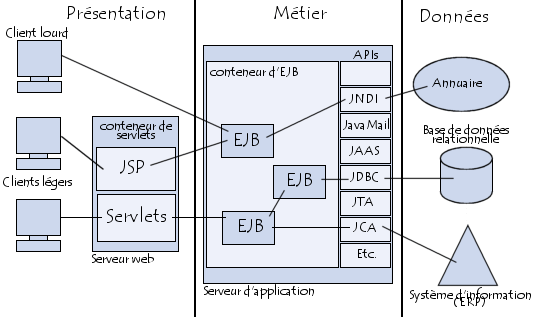
\includegraphics[scale=0.65]{architecture_JEE.png}
   	\caption{Diagramme issu de \url{www.commentcamarche.net}}
    \label{reference1}
\end{figure}
\bigskip

%\textbf{debug : Expliquer l'image}\\
%Et dans la figure  \ref{reference1}\footnote{Diagramme issu de \url{}}
Construit sur la plateforme de Java 2 édition standard (Java SE), la plateforme Java EE ajoute certaines fonctionnalités nécessaires pour fournir une plateforme complète, stable, sécurisée et rapide de Java au niveau entreprise. 
Dans la mesure où J2EE s'appuie entièrement sur le Java, il bénéficie des avantages et inconvénients de ce langage, en particulier une bonne portabilité et une maintenabilité du code.\\
\newline
\indent
L'ensemble de l'infrastructure d'exécution Java EE est donc constitué de services (API) et spécifications tels que:
\begin{itemize}
\item HTTP et HTTPS
\item Java Transaction API (JTA)
\item Remote Method Invocation/Internet Inter-ORB Protocol (RMI/IIOP)
\item Java Interface Definition Language (Java IDL)
\item Java DataBase Connectivity (JDBC)
\item Java Message Service (JMS)
\item Java Naming and Directory Interface (JNDI)
\item API JavaMail et JAF (JavaBeans Activation Framework)
\item Java API for XML Processing (JAXP)
\item Java EE Connector Architecture
\item Gestionnaires de ressources
\item Entreprise Java Beans (EJB)
\item Java Server Pages (JSP)
\item Servlet
\item Java API for XML Web Services (JAX-WS, anciennement JAX-RPC)
\item SOAP with Attachments API for Java (SAAJ)
\item Java API for XML Registries (JAXR)\\
\end{itemize}
Dans le cadre de notre application, seule une sous-partie de ces composants a été utilisée, tels que les servelets, les JSP, JavaMail ou encore JDBC avec Hibernate.\\
\newline
\indent
L'architecture J2EE repose sur des composants distincts, interchangeables et distribués, ce qui signifie notamment :
\begin{itemize}
\item qu'il est simple d'étendre l'architecture 
\item qu'un système reposant sur J2EE peut posséder des mécanismes de haute-disponibilité afin de garantir une bonne qualité de service 
\item que la maintenabilité des applications est facilitée
\end{itemize}
\bigskip

% === avantages
Ces outils favorisent l'interaction avec, d'une part, le solveur, et d'autre part, la base de données. Cela constitue un avantage majeur de notre application. Java EE regroupe donc nativement ces libraires dans un endroit unique. Ainsi, il n'est plus utile  de devoir faire face à des implémentations complexes.
\newline
\indent
De plus, la cohérence du programme favorise la maintenance de celui-ci. Et ce choix favorise le debuggage de l'application.\\
\newline
\indent
Bien qu'ayant déjà utilisé et programmé en Java SE, nous ne nous étions jamais retrouvés confronté au Java Entreprise Edition. La différence entre ceux-ci se trouve surtout dans la complexité de leur utilisation. 
\newline
\indent
Le java SE ayant une approche plus orientée desktop. A contrario, le Java EE propose des outils avancés permettant de faire des applications internet (notamment web, mail, etc.) nécessitant un temps d'apprentissage et d'adaptation plus long. Utiliser du Java EE nous a permis d'en apprendre plus sur ce langage fort demandé en entreprise. En effet, il nous a paru important de connaître ce langage car il constitue un atout majeur pour un développeur.
\newline
\indent
Pour le log des données côté serveur, nous avons également utilisé log4j qui nous à permis de faciliter le travail de debuggage l'application.

\subsection{Hibernate}

Pour pouvoir communiquer avec notre base de données à partir de notre code java, nous avons, dans un premier temps, utilisé JDBC. Ensuite, dans un paradigme objet, nous avons  choisi d'utiliser Hibernate comme une couche supérieure à JDBC. Hibernate permettant de pouvoir transformer les tables en objets, celui-ci offre une bonne cohérence avec l'application.\\
\newline
\indent
Hibernate est un framework libre, appellé framework de  \enquote{mapping objet-relationnel} ou encore de \enquote{persistance objet des données} (voir Figure \ref{reference2}). 
\newline
\indent
Cela permet donc à la couche applicative de notre programme de traiter les données venant de la base de données comme des objets, fournissant un mapping entre le relationel et l'orienté objet.
\newline
\indent
 La base de données peut être traitée avec les avantages de l'orienté objet (comme le polymorphisme, l'héritage, etc.). Le lien entre les classes et la source physique des données  est défini au sein d'un fichier xml. Ainsi, il s'agit effectivement d'un mapping objet-relationnel.
 \newline
 \indent
Cela nous à donc permis de gérer notre base de données dans un paradigme orienté objet comme le reste de l'application.
\begin{figure}[!h]
    \center
   	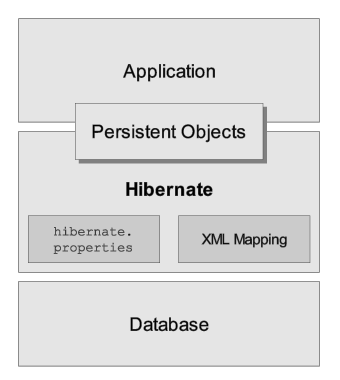
\includegraphics[scale=0.65]{schema_hibernate.png}
   	\caption{Diagramme issu de \url{www.hibernate.org}}
    \label{reference2}
\end{figure}

Un autre avantage recherché par cette solution réside dans son indépendance par rapport à la base de données qui le rend entièrement portable, et cela sans aucune modification du code. Ainsi, comme évoqué précédemment, notre application peut tourner sur 221 base de données différentes.  En effet, notre application, après avoir configuré ses crédentials dans le fichier de configuration de Hibernate, se chargera de créer l’entièreté des tables et la structure de la base de données.\\
 \newline
 \indent
Théoriquement il aurait donc été possible d'envoyer directement un objet "hibernate" (représentant par exemple une table de notre base de données) à GWT donc à l'utilisateur côté client. Cependant, cet aspect reste théorique comme stipulé dans la documentation de GWT\footnote{\url{http://developers.google.com/web-toolkit/articles/using\_gwt\_with\_hibernate}}.
\newline
\indent
En effet, une SerializationException est levée à chaque fois qu'un type transféré via RPC n'est pas sérialisable. La définition de la sérialisibilité signifie ici que le mécanisme RPC - GWT sait comment sérialiser et désérialiser le type de byte code au format JSON et vice-versa.
\newline
\indent
Le problème vient du fait que Hibernate modifie les objets afin de les rendre persistants\footnote{Pour être exact, c'est la librairie Javassist qui se charge de réécrire le byte code de ces objets pour les rendre persistants.}. Au moment du transfert de l'objet, une serialisation est tentée, mais l'objet n'étant pas le même (car modifié par javassist), il ne peut être sérialisé par RPC-GWTP.
\newline
\indent
Pour répondre à cette difficulté majeure, il a été nécessaire d'ajouter des classes de type DTO\footnote{Data Transfer Object}, qui, étant sérialisables, ont pu servir de communication entre la partie cliente et serveur.\\
\newline
\indent
À noter que Hibernate propose son propre langage de requête HQL\footnote{Hibernate Query Language}, syntaxiquement proche du SQL, qui lie vision objet et vision relationnelle\footnote{\url{https://docs.jboss.org/hibernate/orm/3.3/reference/en/html/queryhql.html}}. 

%Hibernate possédant sont propre langage de requête HQL \footnote{Hibernate Query Language}, d'apparence similaire au SQL, mais pleinement orienté Object et comprenant des notions comme l'inhéritance ou de polymorphisme\footnote{\url{https://docs.jboss.org/hibernate/orm/3.3/reference/en/html/queryhql.html}}. Nous n'avons pas pu tirer pleinement avantages et n'étant pas habituer à ce genre de pratique, il a été parfois déroutant d'utiliser un langage mélangeant le SQL et les notions d'orienté objet.

